\documentclass[10pt, a4paper]{scrartcl}

\usepackage{vorschule}
\usepackage[
	typ=ab,
	fach=Informatik,
	lerngruppe={Q2-GK},
	nummer=II.1,
	module={Symbole,Lizenzen},
	seitenzahlen=keine,
	farbig,
	lizenz=cc-by-nc-sa-4,
]{schule}

\usepackage[
	kuerzel=Ngb,
	reihe={Rechnernetze},
	version={2020-10-27},
]{ngbschule}

\author{J. Neugebauer}
\title{Grundlagen der Datenübertragung}
\date{\Heute}

\setzeAufgabentemplate{ngbnormal}

\newcommand{\letter}[2][1.5cm]{#2 $\Rightarrow$ \luecke{#1}}

\begin{document}
\ReiheTitel

Zwischen den beiden Wüstenstädten \emph{New Town} und \emph{Gold City} wurde eine Telegrafenleitung eingerichtet. Diese Leitung besteht aus einem Draht, mit dem auf Tastendruck von beiden Enden aus eine Signallampe zum Brennen gebracht werden kann. Neben der Signallampe verfügen beide Endgeräte über einen Taktgeber, ein Signal, das synchronisiert im Sekundentakt blinkt.

\begin{multicols}{2}\centering
	\vspace*{2mm}
	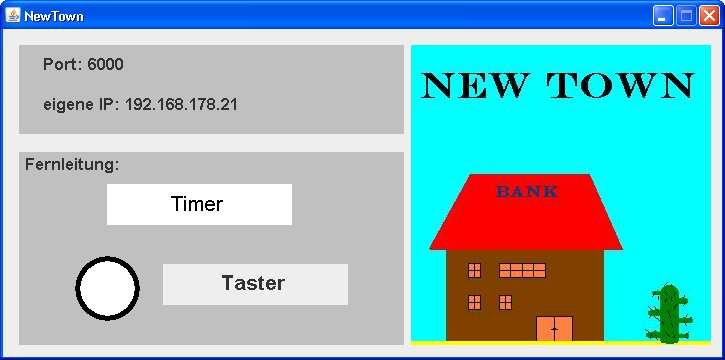
\includegraphics[width=.8\columnwidth]{Q2-GK-AB.II.1-Abb_New Town.png}

	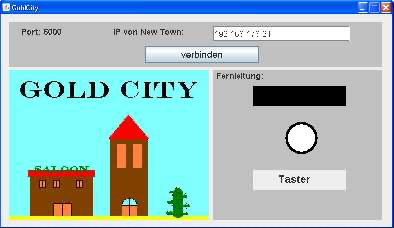
\includegraphics[width=.8\columnwidth]{Q2-GK-AB.II.1-Abb_Gold City.png}
\end{multicols}

\begin{aufgabe}
	Über die Leitung sollen nun Nachrichten wie \enquote{Gold gefunden am Silberberg} oder \enquote{Brauche Männer zum Abbauen} gesendet werden können.

	\begin{teilaufgaben}
		\teilaufgabe Vereinbart zu zweit eine mögliche Codierung der Buchstaben, so dass man die Nachrichten über die eine Leitung verschicken könnte.

		\teilaufgabe Wandelt gemeinsam den Satz \enquote{Gold gefunden} um.
	\end{teilaufgaben}
\end{aufgabe}

Zeichencodierung, auf die ihr beide euch geeinigt habt:
\begin{rahmen}
\begin{multicols}{5}
	\letter{A}

	\letter{B}

	\letter{C}

	\letter{D}

	\letter{E}

	\letter{F}

	\letter{G}

	\letter{H}

	\letter{I}

	\letter{J}

	\letter{K}

	\letter{L}

	\letter{M}

	\letter{N}

	\letter{O}

	\letter{P}

	\letter{Q}

	\letter{R}

	\letter{S}

	\letter{T}

	\letter{U}

	\letter{V}

	\letter{W}

	\letter{X}

	\letter{Y}

	\letter{Z}

	\letter[1.1cm]{leer}
\end{multicols}
\end{rahmen}

\begin{aufgabe}
	Startet die beiden Programme \programm{New Town} und \programm{Gold City} aus dem Tauschordner.

	\begin{teilaufgaben}
		\teilaufgabe Probiert die Funktionsweise der beiden Programme aus.

		\teilaufgabe Entwickelt eine \enquote{Kommunikationsregel}, die es euch ermöglicht, Unterhaltungen über das Programm zu führen.
	\end{teilaufgaben}
\end{aufgabe}

\begin{aufgabe}
	Einer von euch wechselt nun seinen Platz, startet irgendwo im Raum einen anderen Computer und öffnet das Programm \programm{Gold City} aus dem Tauschordner. Derjenige von euch, der sitzen geblieben ist, schließt das Programm \programm{Gold City}.

	\begin{teilaufgaben}
		\teilaufgabe Auftrag für den \programm{Gold City}-Partner: Teile deinem Arbeitspartner deine Lieblingsfarbe mit.

		Auftrag für den \programm{New Town}-Partner: Versuche die Lieblingsfarbe deines Arbeitspartners zu verstehen.

		\teilaufgabe Wechsel die Rollen. Der \programm{New Town}-Partner teilt seinem Arbeitspartner sein Lieblingstier mit und dieser versucht es zu erraten.
	\end{teilaufgaben}
\end{aufgabe}

\begin{aufgabe}
	Überarbeitet eure Kommunikationsregel, so dass eine fehlerfreie Kommunikation möglich ist.
\end{aufgabe}

\end{document}
